%%%%%%%%%%%%%%%%%%%%%%%%%%%%%%%%%%%%%%%%%
% Beamer Presentation
% LaTeX Template
% Version 2.0 (March 8, 2022)
%
% This template originates from:
% https://www.LaTeXTemplates.com
%
% Author:
% Vel (vel@latextemplates.com)
%
% License:
% CC BY-NC-SA 4.0 (https://creativecommons.org/licenses/by-nc-sa/4.0/)
%
%%%%%%%%%%%%%%%%%%%%%%%%%%%%%%%%%%%%%%%%%

%----------------------------------------------------------------------------------------
%	PACKAGES AND OTHER DOCUMENT CONFIGURATIONS
%----------------------------------------------------------------------------------------

\documentclass[11pt,]{beamer}
\usepackage[italian]{babel}

\graphicspath{{data/img/}{./}} % Specifies where to look for included images (trailing slash required)

\usepackage{subcaption}
\usepackage{hyperref}
\usepackage{float}
\floatplacement{figure}{H}
\usepackage{tikz}
\usepackage{pgfplots}
\usepgfplotslibrary{groupplots}
\pgfplotsset{compat=1.18}
\usepackage{amsmath, amsthm, amssymb, amsfonts}

\usepackage{booktabs} % Allows the use of \toprule, \midrule and \bottomrule for better rules in tables

\usetheme{Rochester}
\usefonttheme{default}

\usepackage{palatino} % Use the Palatino font for serif text

\useinnertheme{circles}

%----------------------------------------------------------------------------------------
%	PRESENTATION INFORMATION
%----------------------------------------------------------------------------------------

\title[]{Modelli di traffico per la formazione della congestione su una rete stradale} % The short title in the optional parameter appears at the bottom of every slide, the full title in the main parameter is only on the title page

\author[Gregorio Berselli]{Gregorio Berselli} % Presenter name(s), the optional parameter can contain a shortened version to appear on the bottom of every slide, while the main parameter will appear on the title slide

\institute[UniBO]{Laurea in Fisica \\ \smallskip Universit\`a di Bologna} % Your institution, the optional parameter can be used for the institution shorthand and will appear on the bottom of every slide after author names, while the required parameter is used on the title slide and can include your email address or additional information on separate lines

\date[22 luglio 2022]{22 luglio 2022} % Presentation date or conference/meeting name, the optional parameter can contain a shortened version to appear on the bottom of every slide, while the required parameter value is output to the title slide

%----------------------------------------------------------------------------------------

\begin{document}

%----------------------------------------------------------------------------------------
%	TITLE SLIDE
%----------------------------------------------------------------------------------------

\begin{frame}
	\titlepage % Output the title slide, automatically created using the text entered in the PRESENTATION INFORMATION block above
	\begin{columns}[c]
		\begin{column}{0.55\textwidth}
			
		\end{column}
		\begin{column}{0.45\textwidth}
			\raggedleft
			\scriptsize
			Relatore: Prof. Armando Bazzani \\ \smallskip
			Correlatore: Dott. Alessandro Fabbri
		\end{column}
	\end{columns}
\end{frame}


\begin{frame}
	\frametitle{Congestioni su network stradale}
	\begin{block}{Definizione}
		Diminuzione della qualit\`a del trasporto del network.
	\end{block}
	\vspace{10mm}
	PROBLEMA: studio della dinamica di formazione delle congestioni su network stradale\\ \smallskip
	IDEA: modello di simulazione di un network stradale basato su una dinamica di optimal velocity e una dinamica di incrocio
\end{frame}

\begin{frame}{Diagrammi Fondamentali Macroscopici}
	\begin{columns}[c]
		\begin{column}{.6\textwidth}
			\begin{figure}
				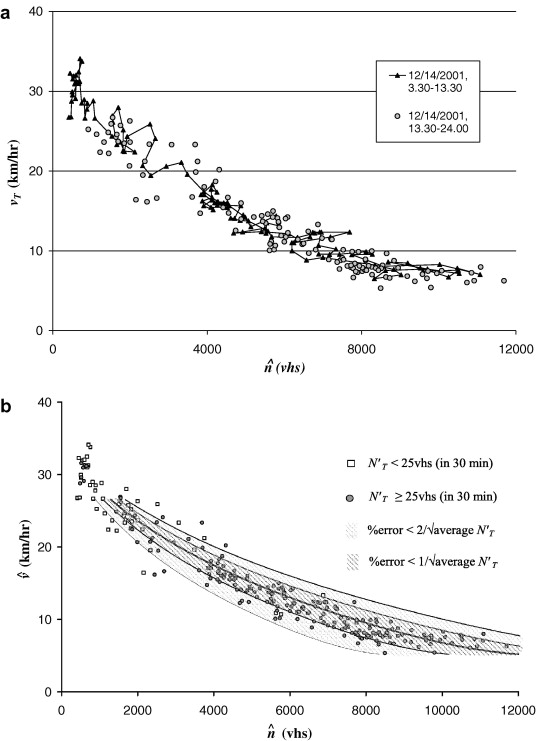
\includegraphics[width=.83\linewidth]{daganzo2.jpg}
			\end{figure}
		\end{column}
		\begin{column}{.4\textwidth}
			\begin{block}{Relazione fondamentale}
				\begin{equation*}
					\Phi=\rho v
				\end{equation*}
			\end{block}
			\vspace{10mm}
			Referenza: \\ \emph{Existence of urban-scale macroscopic fundamental
			diagrams: Some experimental findings}.
		\end{column}	
	\end{columns}
\end{frame}

\begin{frame}
	\frametitle{Modello - Dinamica veicolare: optimal velocity}
	\begin{figure}
		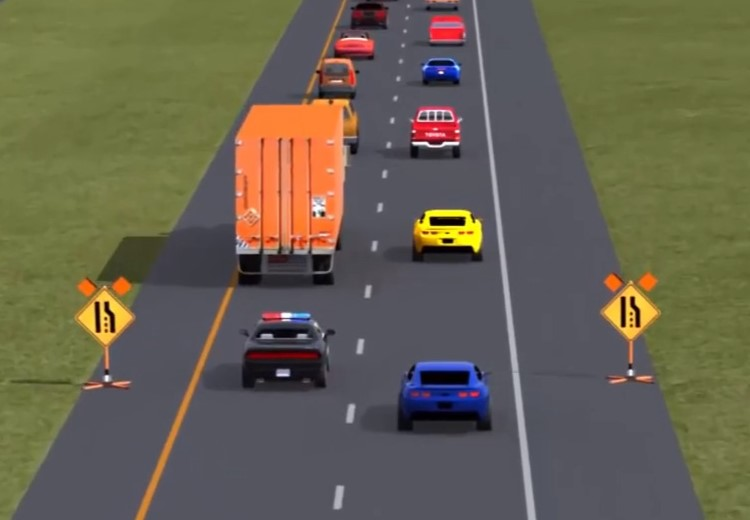
\includegraphics[width=.33\textwidth]{cars.jpg}
	\end{figure}
	\begin{block}{Velocit\`a di immissione}
		\begin{equation*}
			v(t) = v_{max}\left(1-k\frac{\rho(t)}{\rho_{max}}\right)
		\end{equation*}
	\end{block}
	\vspace{10mm}
	La densit\`a stabilisce il \emph{tempo di percorrenza}.	
\end{frame}

\begin{frame}
	\frametitle{Modello - Dinamica agli incroci}
	\begin{figure}
		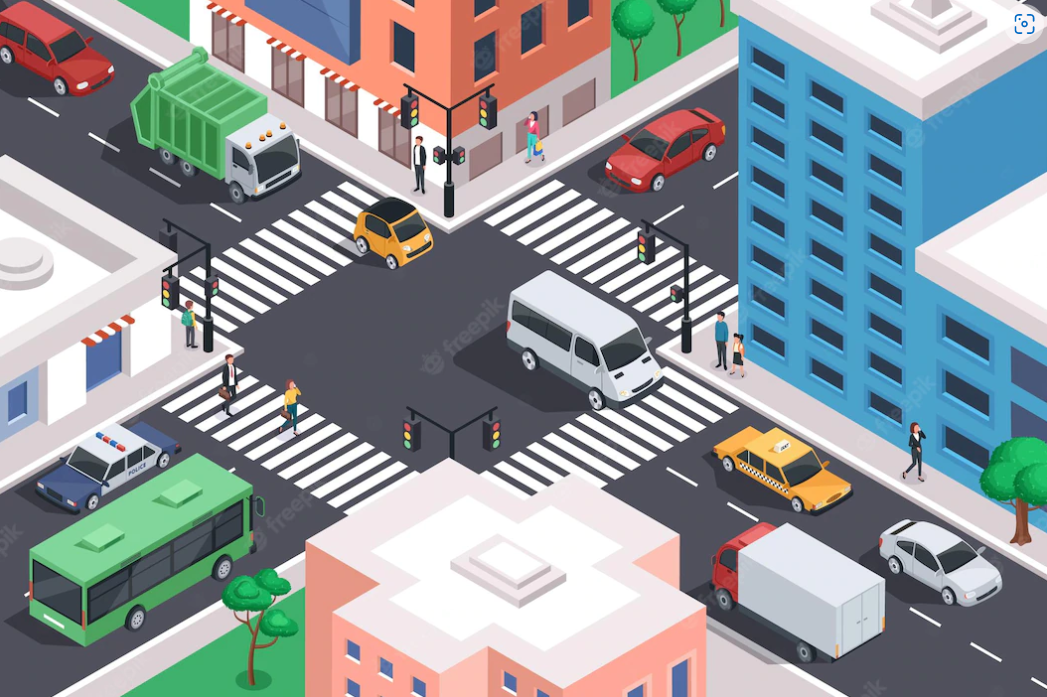
\includegraphics[width=.4\textwidth]{intersection.png}
	\end{figure}
	\begin{itemize}
		\item Se la \emph{penalit\`a temporale} \`e nulla si \`e giunti ad un incrocio
		\item In base al \emph{best path} viene scelta la prossima strada in cui immettersi, in particolare:
			\begin{enumerate}
				\item se vuota, il veicolo si immette e gli viene assegnata una nuova velocit\`a
				\item se piena, il veicolo rimane fermo all'incrocio e ``perde'' uno step temporale
			\end{enumerate}
	\end{itemize}
	
\end{frame}


\begin{frame}
	\frametitle{Simulazioni} % Slide title, remove this command for no title
	
		\begin{block}{Parametri del modello}
			\begin{itemize}
				\item Lunghezza strade: 500 m
				\item Lunghezza veicoli: 8 m
				\item Numero di incroci: 120
				\item Numero di strade: 436
				\item Veicoli immessi: $\sim 10^4$
				\item Velocit\`a massima: 50 km/h (per ogni strada)
				\item Velocit\`a minima: 25\% della velocit\`a massima
			\end{itemize}
			
		\end{block}	
\end{frame}

\begin{frame}
	\frametitle{Rete stradale e domanda di mobilit\`a} % Slide title, remove this command for no title
	\centering
	\begin{figure}
		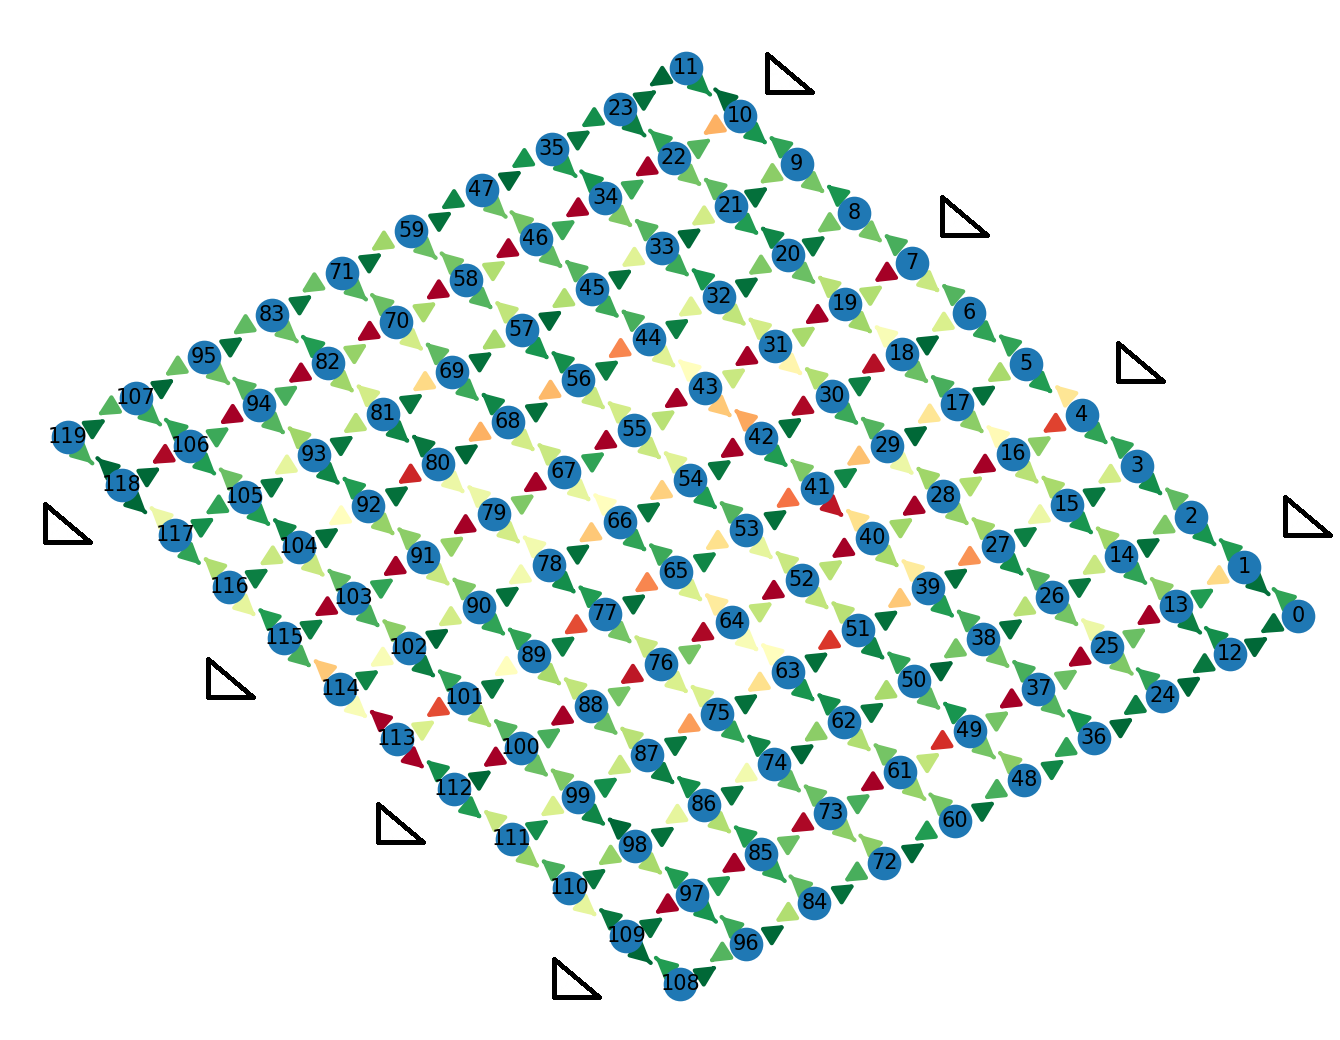
\includegraphics[width=.75\textwidth]{example.png}
	\end{figure}
	\scriptsize
	Scala cromatica da verde scuro (densit\`a nulla) a rosso scuro (densit\`a massima)
\end{frame}


\begin{frame}
	\frametitle{Distribuzioni della congestione in diversi regimi}
	\begin{figure}[H]
		\begin{tikzpicture}[scale=0.69]
			\begin{axis}[ybar interval,
			every tick label/.append style={font=\tiny},
			area style,
			width = 0.75\textwidth,
			height = 0.75\textwidth,
			xlabel = {$\rho$ / $\rho_{max}$},
			ylabel = {Frequenza},
			ymax=0.8,]
			\addplot+[
			ybar interval,
			mark=no,
			line width = 1.25pt
			] plot file {./data/constant_homo/7200_den.dat};
			\addplot[
			domain=0:1.1,
			smooth,
			color=green,
			line width=1.5pt
			] {0.6551*exp(-(6.98*(x+0.05)))};
			\end{axis}
		\end{tikzpicture}
		\begin{tikzpicture}[scale=0.69]
			\begin{axis}[ybar interval,
			every tick label/.append style={font=\tiny},
			area style,
			width = 0.75\textwidth,
			height = 0.75\textwidth,
			xlabel = {$\rho$ / $\rho_{max}$},
			ymax=0.8,]
			\addplot+[
			ybar interval,
			mark=no,
			line width = 1.25pt
			] plot file {./data/peaked_homo/5800_den.dat};
			\addplot[
			domain=0:0.8,
			smooth,
			color=green,
			line width=1.5pt
			] {0.3239*exp(-(3.7*(x+0.05)))};
			\addplot[
			domain=0.8:1.1,
			smooth,
			color=red,
			line width=1.5pt
			] {3*10^(-8)*exp(14.484*(x+0.05))};
			\end{axis}
		\end{tikzpicture}
		\caption{\emph{Distribuzione rapporto densit\`a / densit\`a massima per network non congestionato (sinistra) e congestionato (destra) con interpolazioni esponenziali.}}
		\end{figure}
	
\end{frame}

\begin{frame}
	\frametitle{Fenomeno di isteresi}
	Congestione: diminuzione repentina del flusso medio \bigskip
	\begin{figure}[H]
		\begin{tikzpicture}[scale=0.63]
			\definecolor{dkgreen}{cmyk}{0.5,0.1,0.5,0.4};
			\begin{axis}[
			grid = both,
			major grid style = {lightgray},
			minor grid style = {lightgray!25},
			width = 0.75\textwidth,
			height = 0.5\textwidth,
			xlabel near ticks,
			xmax = 0.5,
			xlabel = {Tempo (h)},
			ylabel = {Flusso (veh/h)},]
			\addplot[
			mark size=1,
			draw=dkgreen,
			mark=o,
			style=very thick] file {./data/peaked_homo/q-t_load.dat};
			\addplot[
			mark size=1,
			draw=red,
			mark=o,
			style=very thick] file {./data/peaked_homo/q-t_unload.dat};
			\addplot[
			mark size=1,
			draw=dkgreen,
			mark=o,
			style=very thick] file {./data/peaked_homo/q-t_unload2.dat};
			\end{axis}
			\end{tikzpicture}
		\begin{tikzpicture}[scale=0.63]
			\definecolor{dkgreen}{cmyk}{0.5,0.1,0.5,0.4};
			\begin{axis}[
			grid = both,
			major grid style = {lightgray},
			minor grid style = {lightgray!25},
			width = 0.75\textwidth,
			height = 0.5\textwidth,
			ylabel near ticks,
			xlabel near ticks,
			xlabel = {Densità (veh/km)},]
			\addplot[
			mark size=1,
			draw=dkgreen,
			mark=o,
			style=very thick] file {./data/peaked_homo/q-k_load.dat};
			\addplot[
			mark size=1,
			draw=red,
			mark=o,
			style=very thick] file {./data/peaked_homo/q-k_unload.dat};
			\addplot[
			mark size=1,
			draw=dkgreen,
			mark=o,
			style=very thick] file {./data/peaked_homo/q-k_unload2.dat};
			\end{axis}
		\end{tikzpicture}
		\caption{\emph{Variazione del flusso medio nel tempo (sinistra) e diagramma temporale flusso/densit\`a (destra).}}
		\end{figure}
\end{frame}

\begin{frame}
	\frametitle{Conclusioni}
	\begin{block}{Riscontri positivi}
		\begin{itemize}
			\item Evidenziate le principali dinamiche
			\item Congestioni \emph{localizzate} nello spazio
		\end{itemize}
	\end{block}

	\bigskip \bigskip

	\begin{block}{Necessit\`a}
		\begin{itemize}
			\item Rete pi\`u realistica da inserire
			\item Confronto con dati reali
		\end{itemize}
	\end{block}
\end{frame}

%----------------------------------------------------------------------------------------
%	CLOSING SLIDE
%----------------------------------------------------------------------------------------

\begin{frame}[plain] % The optional argument 'plain' hides the headline and footline
	\begin{center}
		{\Huge Grazie per l'attenzione}
		
		\bigskip\bigskip % Vertical whitespace
		
		{\LARGE Riferimenti principali:}
		
		\bigskip
		\small

		Nikolas Geroliminis, Carlos F. Daganzo ``Existence of urban-scale macroscopic fundamental diagrams: Some experimental findings.'' (2008), https://doi.org/10.1016/j.trb.2008.02.002.
		
		\bigskip
		
		Gazis, Denos C. ``The origins of traffic theory.'' (2002): 69-77.
		
		\bigskip
		
		Park, S., Rakha, H. and Guo, F. ``Calibration issues for multistate model of travel time reliability.'' (2010).
	\end{center}
\end{frame}

\begin{frame}[plain]{}
\end{frame}

\begin{frame}
	\frametitle{Evoluzione temporale completa}
	\centering
	\begin{figure}[H]
		\begin{tikzpicture}
			\definecolor{dkgreen}{cmyk}{0.5,0.1,0.5,0.4};
			\begin{axis}[
			grid = both,
			major grid style = {lightgray},
			minor grid style = {lightgray!25},
			width = 0.75\textwidth,
			height = 0.5\textwidth,
			xlabel near ticks,
			xlabel = {Tempo (h)},
			ylabel = {Flusso (veh/h)},]
			\addplot[
			mark size=1,
			draw=dkgreen,
			mark=o,
			style=very thick] file {./data/peaked_homo/q-t_load.dat};
			\addplot[
			mark size=1,
			draw=red,
			mark=o,
			style=very thick] file {./data/peaked_homo/q-t_unload.dat};
			\addplot[
			mark size=1,
			draw=dkgreen,
			mark=o,
			style=very thick] file {./data/peaked_homo/q-t_unload2.dat};
			\end{axis}
			\end{tikzpicture}
		\caption{\emph{Variazione del flusso medio nel tempo.}}
		\end{figure}
\end{frame}

\begin{frame}
	\frametitle{Sistema congestionato}
	\centering
	\begin{figure}
		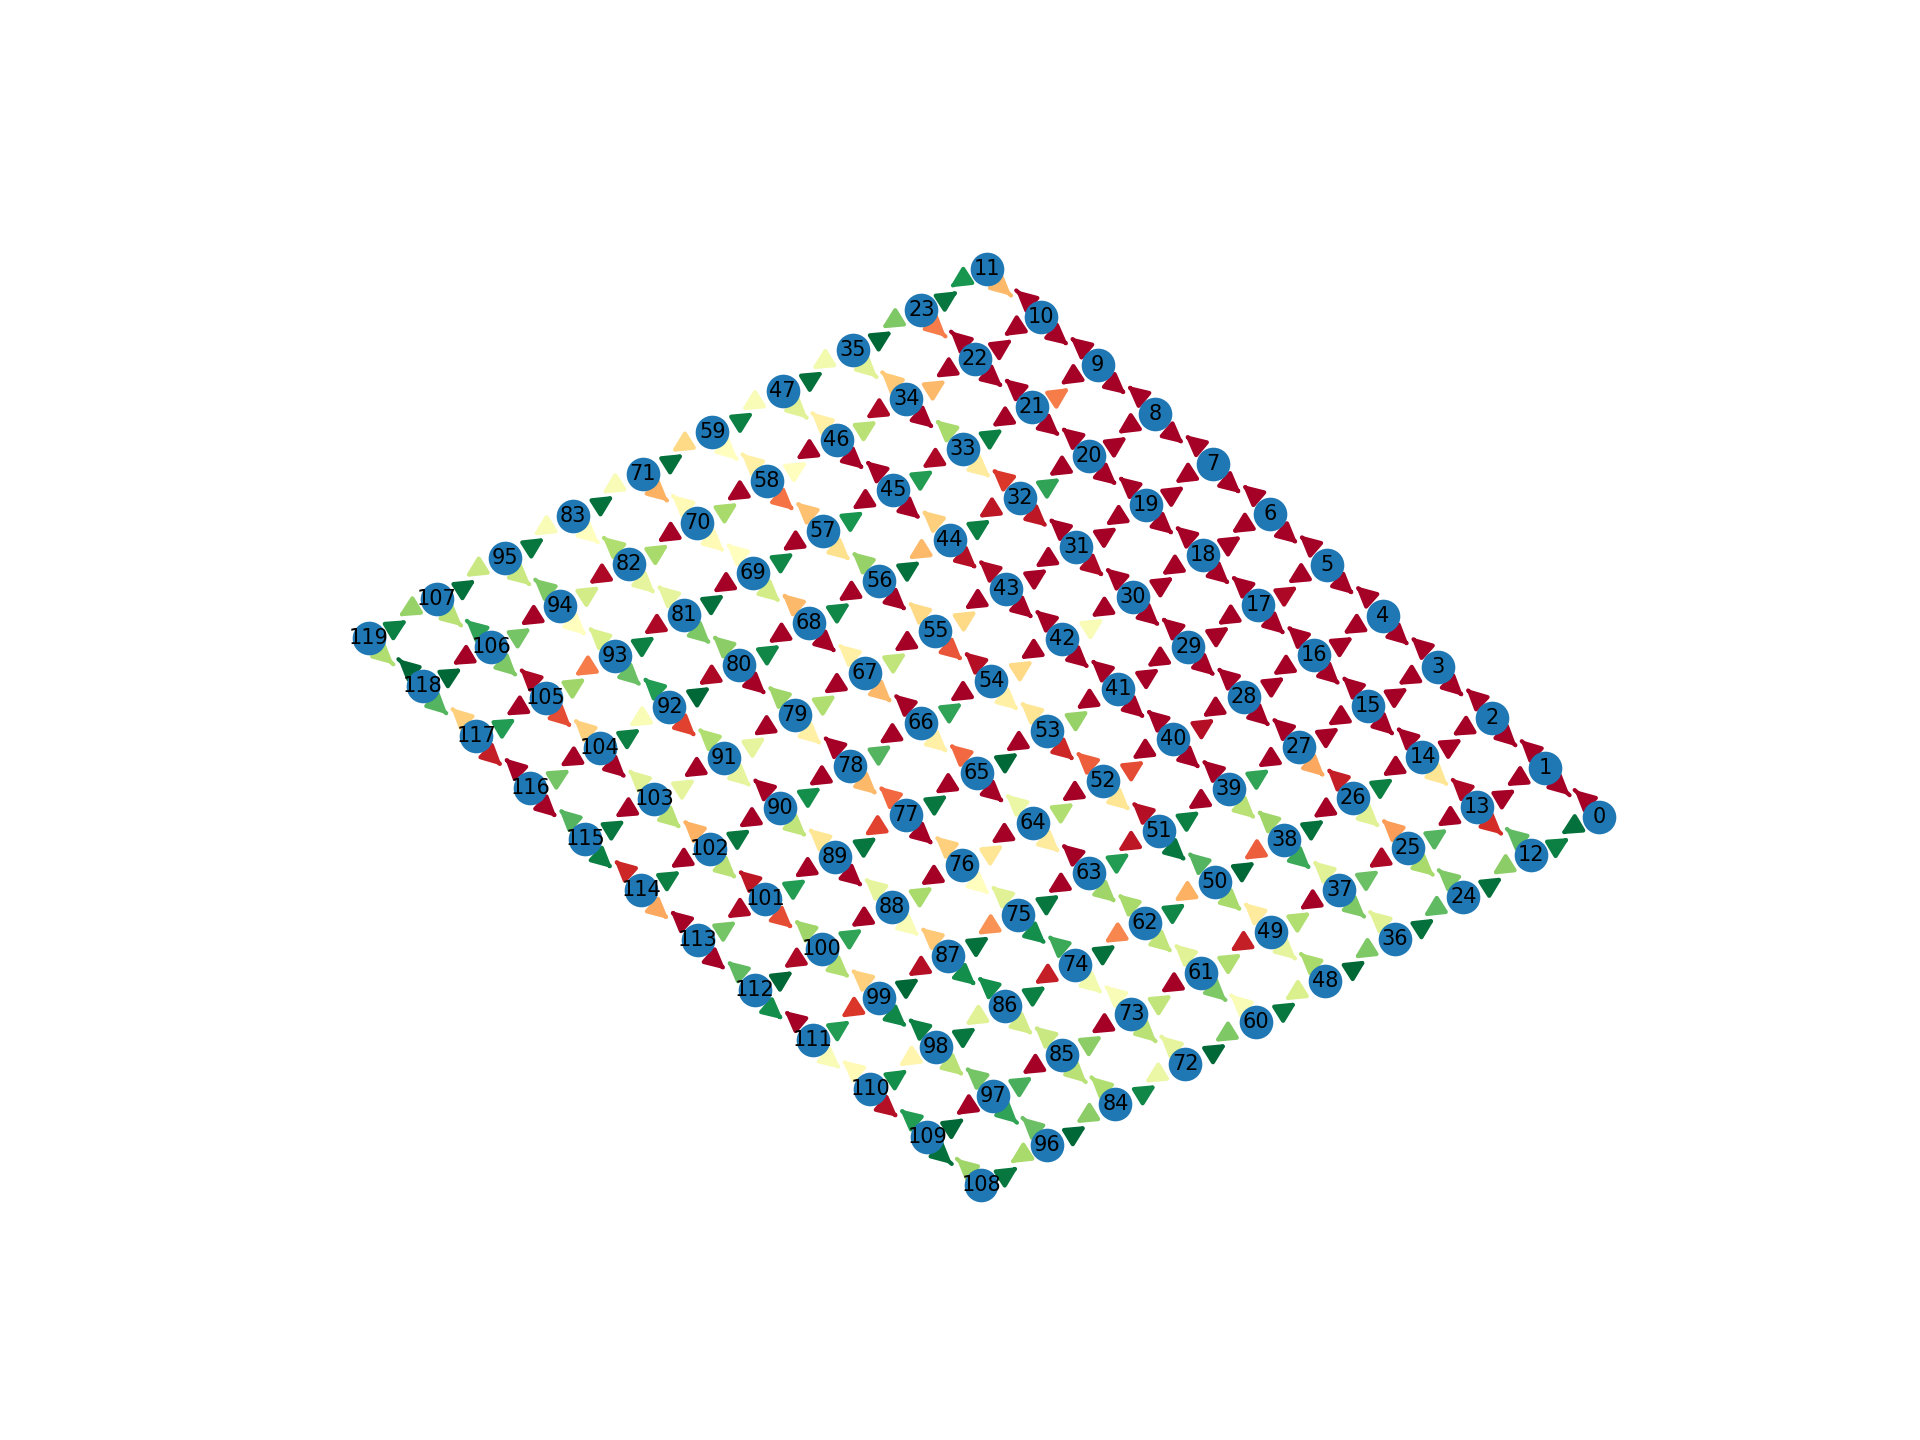
\includegraphics[width=.8\textwidth, trim={12.5cm 8cm 10cm 8cm},clip]{congested_flow.png}
	\end{figure}
\end{frame}

\begin{frame}
	\frametitle{Distribuzioni della congestione in diversi regimi - Log Scale}
	\begin{figure}[H]
		\begin{tikzpicture}[scale=0.69]
			\begin{axis}[ybar interval,
			every tick label/.append style={font=\tiny},
			area style,
			width = 0.75\textwidth,
			height = 0.75\textwidth,
			xlabel = {$\rho$ / $\rho_{max}$},
			ylabel = {Frequenza},
			ymode=log,
			log origin=infty,]
			\addplot+[
			ybar interval,
			mark=no,
			line width = 1.25pt
			] plot file {./data/constant_homo/7200_den.dat};
			\addplot[
			domain=0:1.1,
			smooth,
			color=green,
			line width=1.5pt
			] {0.6551*exp(-(6.98*(x+0.05)))};
			\end{axis}
		\end{tikzpicture}
		\begin{tikzpicture}[scale=0.69]
			\begin{axis}[ybar interval,
			every tick label/.append style={font=\tiny},
			area style,
			width = 0.75\textwidth,
			height = 0.75\textwidth,
			xlabel = {$\rho$ / $\rho_{max}$},
			ymode=log,
			log origin=infty,]
			\addplot+[
			ybar interval,
			mark=no,
			line width = 1.25pt
			] plot file {./data/peaked_homo/5800_den.dat};
			\addplot[
			domain=0:0.8,
			smooth,
			color=green,
			line width=1.5pt
			] {0.3239*exp(-(3.7*(x+0.05)))};
			\addplot[
			domain=0.8:1.1,
			smooth,
			color=red,
			line width=1.5pt
			] {3*10^(-8)*exp(14.484*(x+0.05))};
			\end{axis}
		\end{tikzpicture}
		\caption{\emph{Distribuzione rapporto densit\`a / densit\`a massima per sistema non congestionato (sinistra) e congestionato (destra) con interpolazioni esponenziali.}}
		\end{figure}
	
\end{frame}

\end{document} 